\chapter{绪论}

%%%%%%%%%%%%%%%%%%%%%%%%%%%%%%%%%%%%%%%
%-----------------------------------     研究背景和意义     -----------------------------------%
%%%%%%%%%%%%%%%%%%%%%%%%%%%%%%%%%%%%%%%
本章内容主要介绍论文的研究背景和意义、研究现状、论文的工作与创新点和论文的组织结构
\section{研究背景和意义}
在飞速发展的互联网影响下,越来越多的网络数据积累下来。网络结构数据涉及的领域也越来越广,不同领域的应用都少不了对网络类数据的挖掘,比如社交网络、通信网络、生物蛋白质网络,金融交易网络,这些网络都是用来表示一个个复杂系统,在网络中,节点用来表示复杂系统的个体或实体,连边表示个体或实体间的相互关系,比如社交网络中的相互关注、互为好友,通信网络中的相互连接,生物蛋白质之间的相互作用等。随着覆盖领域的扩大,越来越多的现实应用需要挖掘网络中的信息,比如社交网络Twitter\footnote{www.twitter.com}的推荐系统需要通过挖掘网络信息而实现给用户推荐符合用户偏好的推文,广告精准投放系统中通常需要将社交网络中的用户分成不同的社区来提高精度。因此,挖掘网络中的信息是非常具有实际价值的。

\begin{figure}
	\centering
	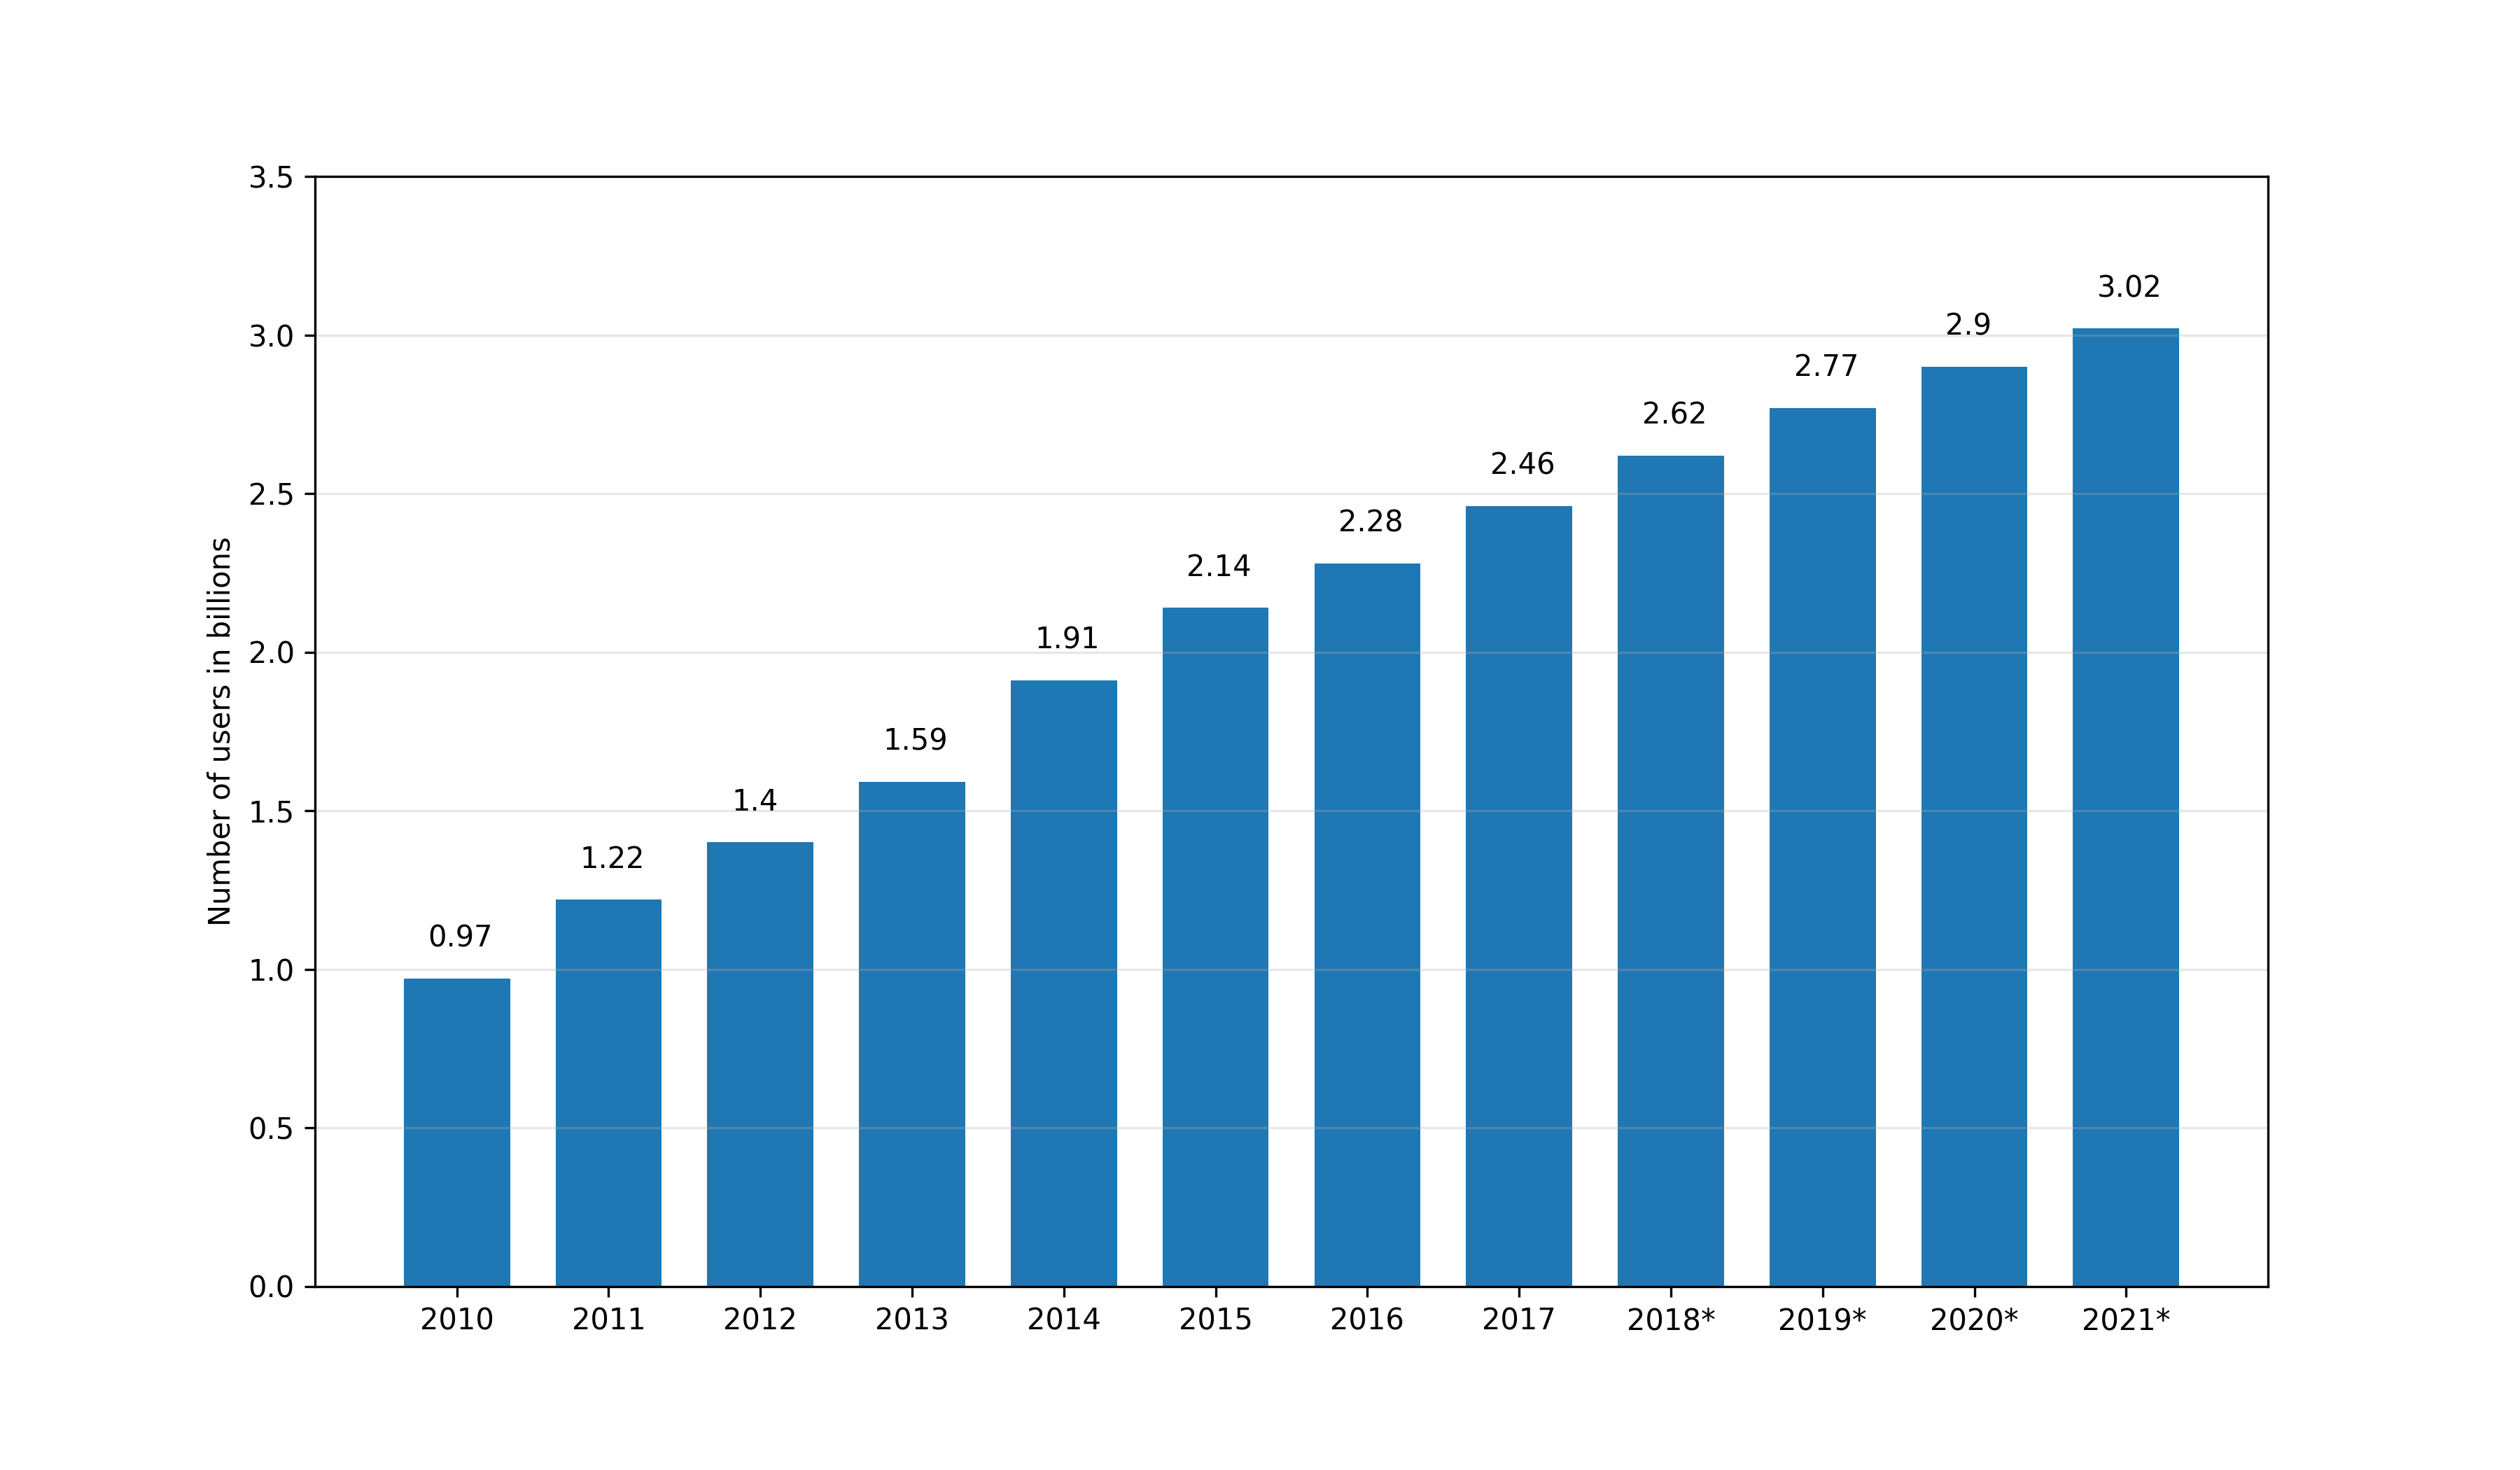
\includegraphics[width=5.5in]{figures/social_media_stat}
	\caption{2010-2021年全球社交媒体用户总数量(以10亿为单位)| 图自:Stataista。}
\end{figure}

在以Facebook\footnote{www.facebook.com}、Twitter、微信\footnote{weixin.qq.com}、微博\footnote{www.weibo.com}为代表的大型在线网络中,网络中的节点数以亿计,网络结构非常复杂,对于巨大规模的高维数据的分析和处理都离不开巨大的储存的计算消耗,从中进行挖掘任务直观上复杂度非常高,而且面对高维数据有可能会产生维数灾难\cite{bellman2015adaptive}(curse of dimensionality)。所谓维数灾难,就是在没有简化参数搜索空间的情况下,对于多参数的函数进行最优化学习时,如果需要得到稳定的参数学习效果,学习样本需要跟随着参数量的增加而指数级的增长,这对于参数学习来说无疑显著地增加了成本。这些问题的原理是因为随着参数量的增加,假设空间不断扩大使得真正有用的数据在空间中的表示非常稀疏。事实上,往往在对事情进行描述刻画的时候,有一种直观的体验,那就是关键特征的选择性描述就会达到足够好的表达效果,而不需要将事物的方方面面描述出来,这样也从另一方面减少信息被淹没的可能,也就是从稀疏的表征空间中得到了真正有用的数据,这种直观的体验引出了数据降维技术。通过数据降维技术可以将特征温度降到合适的量级,可以明显地提高数据分析时候的存储和计算消耗,对于大规模高维数据分析是必不可少的技术手段。

类比在对于网络的描述,也可以不用邻接矩阵的形式将每个节点的所有邻居都描述出来,抽象出特定的节点表征形式也可以达到包含足够的网络信息。因此,在网络挖掘研究任务中,一个基础的研究工作就是学习有效的节点表征,将网络映射到一个低维向量空间中\cite{chang2015heterogeneous},也就是学习每个节点的低维向量表示,这个过程一般称为图表征(Network Embedding/Representation)。图表征算法属于表示学习或称为特征学习,目标就是自动学习从原始特征表示到新的特征表示的一种变换,使得新的特征适合后续的机器学习任务。利用节点的向量表示可以结合机器学习方法进行进一步的挖掘,例如信息检索\cite{weiss2009spectral},节点分类\cite{krizhevsky2012imagenet},聚类\cite{ng2002spectral}等。分类算法作为数据挖掘常用的算法,应用在网络研究之中可以用来对网络中的节点进行分类研究。在网络中的节点分类,分为两个不同的研究问题,即单标签分类问题和多标签分类问题。如果样本实例只能属于某一种类别标签,这种分类问题属于单标签分类问题;如果样本实例可能会属于多种类别标签,这种则属于单标签分类问题。这两种问题在网络研究场景下分别对应不同的情况,比如社交网络中每个用户的标签即为用户所属社区,非重叠社区场景对应单标签分类问题,重叠社区场景则对应多标签分类问题。

在具体的应用场景中,网络中的节点除了各自的邻居集合有所差异以外,节点本身也会有着丰富的属性差异,例如:在社交网络中,不同的节点会有不一样的用户名、用户ID、性别、年龄等丰富的属性信息,这些属性信息一定程度上表示用户的属性和性质,这些现实的属性信息在一定程度上回影响局部甚至整体网络的静态属性和动态演化,这些网络一般称之为属性网络。比如,社会网络中互为好友的用户如果有共同的兴趣爱好,那么会更大程度地增强联系。通过对属性信息的处理和分析,可以提取有利于网络挖掘的特征,把网络的拓扑结构信息和节点的属性信息结合起来,可以对后续的学习任务提供更有价值的特征。

除此以外,大部分网络挖掘研究关注的是静态网络。静态网络中节点和边的状态基本不变,而且大部分对于静态网络的研究需要得到完整的网络拓扑结构。与之不同的是,在真实世界中的网络是时刻变化的,新的节点和关系会持续不断加入到网络中,这种网络一般称为流式网络\cite{aggarwal2014evolutionary}。在流式网络中,部分节点的关系是暂时性,比如在邮件或者通信网络中,用户的交互可以用代表节点关系的流数据来表征。持续的流数据需要采用实时的方式来进行分析,全局或者静态的分析手段不再适用。在机器学习领域,对流数据以增量方式进行学习方法称为在线学习或增量学习,就是对新产生的数据样本通过离线训练好的模型进行预测的,同时对离线模型本身也进行更新,从而减少对历史数据重新计算而造成的资源浪费。在对流式网络挖掘和网络演化的研究中,由于网络规模巨大无法将对整个网络进行全局分析,并且要考虑到足够低的时间复杂度,因此对于流式网络的研究非常具有挑战性\cite{zhao2011gsketch,le2012linked}。

%%%%%%%%%%%%%%%%%%%%%%%%%%%%%%%%%%%%%%%
%----------------------------------------     研究现状     ---------------------------------------%
%%%%%%%%%%%%%%%%%%%%%%%%%%%%%%%%%%%%%%%
\section{研究现状}
下面从以下几个方面开始介绍国内外相关研究现状:
\begin{itemize}
\item {图表征学习的意义及相关研究}
\item {属性网络的重要性及相关研究}
\item {增量图表征的相关研究}
\item {增量学习的相关研究}
\end{itemize}

关于图表征算法的研究,最早源自谱聚类(Spectral Clustering )的研究,顾名思义,谱聚类首先是一种聚类方法,具体思想则是通过挑选对应矩阵中的特征值和特征向量来得到节点的表征,谱聚类被广泛地使用在社区发现(Community Detection)\cite{leskovec2010empirical}和图像分割(Image Segmentation)[\cite{shi2000normalized}领域。后2000年有人提出流形学习的方式来实现图表征,主要方式是保证网络结构的局部特性来构建近似网络,将问题转化为特征分解的问题,从而实现映射到低维向量空间的目标;在流形学习中最具代表性的几个算法:局部线性嵌入\cite{roweis2000nonlinear}LLE(Locally Linear Embedding)、等距映射ISOMAP\cite{tenenbaum2000global} (Isometric Feature Mapping)和拉普拉斯特征映射LE\cite{belkin2002laplacian}(Laplacian Eigenmaps)。图表征中的LLE算法,假设在网络的局部领域上任意节点的表征向量应该是欧式的,也就是说表征向量是局部线性的。根据这个假设,任意节点的表征向量都可以用它的邻居以加权的形式线性表示出来,在非平凡解的约束下,可以得到LLE的解,可以看出LLE是一种局部流形学习方法。与此不同的是,等距映射ISOMAP的假设是节点表征向量应该使变换前后距离保持不变,而且等距映射ISOMAP是一种全局流形学习方法。而拉普拉斯特征映射跟类似于LLE算法,基本假设是,网络中连边权重较大的节点之间,表征向量越接近。

在此之后,对于图表征的算法研究开始成为一个新的领域。其中,DeepWalk\cite{perozzi2014deepwalk}引进自然语言处理中的词向量表征算法,通过网络中的随机游走进行网络采样形成类似语料库的路径集,进而实现对网络节点向量表征的学习。2015年,Tang\cite{tang2015line}提出了一种可扩展的图表征算法LINE,其中提出了一阶接近度和二阶接近度(first-order proximity and second-order proximity)来描述网络结构,一阶接近度相当于描述网络中互为邻居的相似程度,论文中以KL散度(Kullback-Leibler divergence)作为距离函数进行描述,二阶接近度则是用来描述网络中存在共同邻居的节点之间的相似程度,同样以KL散度为距离函数,并基于接近度的组合构建图表征算法需要优化的目标函数,进一步通过优化目标函数实现目标。2016年,Grovel\cite{grover2016node2vec}基于DeepWalk的方式改进了随机游走方式,提出node2vec算法,论文中将随机游走过程更改为具有两个自由度的模型,通过这两个参数分别控制广度优先和深度优先,从而保留网络结构的同质性特征或者结构等价性特征。另外,一些基于矩阵分解的算法\cite{ahmed2013distributed,singh2008relational,zhu2007combining}被提出,其中Shenghuo Zhu等基于PCA,NMF方式提出一种改进的矩阵分解方式,同时在目标函数中结合边信息和属性信息。除此之外,Jiezhong Qiu等\cite{qiu2017network}提出以上方法的统一解释,推导出包括DeepWalk,LINE,PTE\cite{tang2015pte},node2vec在内的四种算法的矩阵分解形式。

单纯基于网络结构本身的研究在应用上存在局限性,因为网络中节点会包含丰富的属性信息,如文本,图片等相关信息,除去从文本,图片中提取特征的基本手段外,如何使这些属性信息更有利于网络表征学习过程也具有非常可观的价值。关于属性网络中图表征算法的研究,在Cheng Yang\cite{yang2015network}和Huang\cite{huang2017accelerated}的研究中,提出合并的特征表示方式,将节点的属性特征和网络结构本身的特征结合起来,从而得到更利于节点分类的向量表征形式,Cheng Yang等在TADW(text-associated Deep Walk)中首次提出并证明DeepWalk的矩阵分解形式,结合文本特征构造目标函数,实现将文本特征融入到网络表征中。在2016年,Zhang\cite{zhang2016collective}提出了一种基于判别矩阵分解的方法,在矩阵分解的目标函数中加入分类的经验损失函数,将分类任务和图表征过程结合起来统一优化,使得到的结果在表征足够多信息的同时,具有良好的分类性能。

然而,大部分的网络表征学习研究对象都是静态的网络,实际的网络是处在不断变化和演进中的,Li\cite{li2017attributed}基于动态网络的变化是缓慢且持续的假设,提出了一种动态网络中的网络表征算法,在论文中,采用拉普拉斯特征映射(Laplacian eigenmaps)的目标函数,并结合节点属性向量,计算各节点间的属性相似度,构造类似邻接矩阵的属性相似度矩阵,将属性相似度矩阵与邻居矩阵分别进行特征映射,再通过优化映射将两组特征融合起来;在增量场景下利用矩阵摄动理论推导网络表征中特征值和特征向量的增量,从而可以快速得到新的网络表征。增量网络表征过程一定程度上类似于增量的机器学习过程,但是可以看出流式网络

在互联网技术发展迅猛的当下,业界以几何倍数地积累着越来越多的数据,数据分析和处理就遇到了一些问题。首先,想要获得大量的标注数据是非常耗费资源的,那么人工标注数据这种手段显然是不可行的,采用机器学习算法自动进行预测分析才是首选。而对于机器学习算法而言,数据增长到一定的规模,模型训练的时间会非常长,这会非常影响用户体验,特别是对于线上的程序,以传统方式对模型重新训练几乎是不可能的。另外最重要一点,对于分类模型,如果出现了一个新的类,那么传统的机器学习算法是无法自动识别的。在意识到传统机器学习的这些问题后,Coppock和Freund在1962年提出了增量学习的概念\cite{coppock1962all},或称为在线学习,这两个概念略有区别,但在本文讨论范围内不作区分。区别于传统算法,增量学习应该具有一些特性:首先,分类器根据新的数据会学习新的信息,也就是说模型会根据新数据进行更新;其次,在增量学习时,用于学习的应该只有新的数据,而不是需要整合原始数据和新数据。 根据文献的不同增量学习算法特征,可以将分类问题的增量学习分为三个种类:样本增量学习(Sample Incremental SIL),类别增量学习(Class Incremental Learning)和特征增量学习(Feature Incremental Learning)\cite{zhong2017survey};其中样本增量学习就是假设不断有新的样本加入,同时数据的特征维度,和预测分类数仍保持不变;类别增量学习顾名思义就是假设预测的类别数有可能变化,在新的数据可能会有新类别产生的;特征增量学习就是假设在数据的特征维度在变化。大部分的在线学习算法是基于随机梯度下降(Stochastic Gradient Descent)的改进\cite{hazan2007logarithmic, xiao2010dual, mcmahan2011follow},基于在线梯度下降的算法优点在于精度高,但是局限在于即使加上L1正则(L1-Norm)很难产生真正意义上的稀疏解,同时在一些不可微点的迭代会出现问题。于是基于这些局限,提出了一些能改善稀疏性的方案,最简单的方式是梯度截断(Truncated Gradient),设定一个梯度阈值或者参数阈值,当参数小于阈值时直接设为0;John Duchi和 Yoran Singer\cite{duchi2009efficient}提出了前向后向切分算法FOBOS(Forward Backward Splitting),算法类似于投影梯度下降,但将迭代过程修改成了两步,第一步更新为经验损失函数的梯度下降过程,第二步更新编程求解一个最优化问题,其中第二个最优化问题首先通过L2-norm限制损失迭代结果的范围,其次再增加正则项对模型复杂度进行限制从而达到稀疏结果,从理论上可以证明,第二步的最优化可以使得模型结果具有稀疏性,FOBOS算法使得在线模型具有了可观的稀疏性和不错的精度,FOBOS算法在特定情况下等同于简单的梯度截断方法。Lin Xiao\cite{xiao2010dual}提出了正则对偶平均算法RDA(Regularized Dual Averaging Algorithm),这个算法本身不同于梯度下降方式的学习算法,改成以一个最优化问题进行权重的更新,相当于在某个特征维度的参数累计梯度平均值低于阈值λ后进行截断,通过调节λ可以在稀疏性和精度之间做权衡。从此可以看到基于梯度下降的FOBOS具有较好精度,但是稀疏性不如RDA算法,于是H. Brendan McMahan提出了FTRL(Follow-the-Regularized-Leader)算法\cite{mcmahan2011follow},FTRL算法在L1正则情况下精度和稀疏性都好于前者,从参数更新的形式上看,FTRL优化的最优化问题跟RDA算法只在额外项上存在差异,通过额外项限定新的参数迭代结果不要离上一步的结果太远。另外一个体系是基于SVM(Support Vector Machine)的增量学习方式,Syed等\cite{syed1999incremental}最新提出的增量式方法基于SVM算法的特性,影响分割超平面的是全部的支持向量,而支持向量的个数相对总体样本而言是非常少的,于是Syed等提出在增量学习过程中,对增量的样本和支持向量一起进行重新训练得到新的分类器,循环迭代得到最后的分割超平面,利用支持向量机的特性而设计的这种增量方法提供在处理海量数据是可以为提供不错的优化的,但是模型也存在着明显的局限,那就是数据集特征本身的分布影响着训练过程甚至训练结果的好坏。为了解决数据集特征分布上的差异引起的模型性能,Ruping\cite{ruping2001incremental}在对原始数据子集和新增数据子集采取不一样的方式,通过在目标函数中对不同子集的间隔设置不同的权重,使得数据特征保持良好稳定的分布,通过实验表明,通过调整得到的分割超平面类似于批处理得到的结果。

根据判别误分类的差异,这些算法可以进一步分成软间隔和硬间隔两种。相比之下,软间隔分类器的一个优点是可以减少一部分噪音数据的影响\cite{kivinen2002large}。



%%%%%%%%%%%%%%%%%%%%%%%%%%%%%%%%%%%%%%%
%---------------------------------     本文工作与创新点     ---------------------------------%
%%%%%%%%%%%%%%%%%%%%%%%%%%%%%%%%%%%%%%%
\section{本文工作与创新点}
本文主要研究的问题是在动态变化的增量网络中,进行快速的网络挖掘学习。为此本文将围绕这一个话题展开研究和分析,提出可行的方案框架。本节将对本文的全部工作内容作简明的概括,详细的分析和研究将于后文具体展开。


\subsection{主要工作}
本文的研究工作将着重围绕以下两个研究问题来展开:
\begin{itemize}
\item \textbf{问题1: 如何以增量的形式提取网络特征?}
\item \textbf{问题2: 如何通过通过增量学习?}
\end{itemize}

就\textbf{问题1},本文将从两个步骤来分析和解决。移动应用开发流程通常包括需求分析、开发实现、后期维护等步骤,而其中需求分析和后期维护是本文所关注的两个阶段。需求分析是获得移动应用功能的最初阶段,此时可以通过分析需求文档来获得移动应用的功能需求。由于此类文档通常为内部文件,一般无从获得。为了能够获得类似的文档信息,本文转而分析移动应用的描述信息。因为移动应用的描述通常是对其整体功能的概述,里面包含了移动应用最关键的功能描述,亦是开发者的需求。因此,对于\textbf{问题1},第一步骤将移动应用的描述作为信息源,通过分析其中的功能描述,从而获取开发者的需求。在后期维护中,开发者需要根据市场反馈进行漏洞修复、功能添加等操作。而此时,开发者已有一个初版移动应用或是早期发布的版本,这一已有版本的移动应用便完整地包括了开发者所有的功能需求。通过比较不同移动应用的视图信息,本文发现视图相似的移动应用通常具有类似的功能,相似的移动应用可以从侧面表现目标移动应用的功能信息。因此,第二步骤利用已有版本的移动应用作为信息源,通过分析其视图信息并与相似移动应用比较,从而获取开发者的需求。本文分别从不同角度对开发者需求进行分析和整合,从而协助开发者在不同阶段更高效地开发质量更好的移动应用。

就\textbf{问题2},本文亦分为两个步骤来开展。首先,根据\textbf{问题1}分析所得的移动应用的功能信息,对移动应用进行聚类。为了给开发者推荐合适的第三方库,本文通过分析市场上移动应用使用的第三方库情况,寻找功能类似的移动应用,其所使用的第三方库表征了该第三方库在此类功能中的通用性。因此,通过聚类的方法可以将相似功能的移动应用聚到一起,即整合了同类功能移动应用所使用的第三方库。其次。在此基础上,对于同一类别中的移动应用,本文根据类内每个移动应用与目标移动应用的相似度,以及各个移动应用的评分情况,对类内移动应用进行排序。其中排名最高的若干个移动应用将放入候选池,这些移动应用所使用的第三方库将作为推荐的候选列表,最终将根据各个第三方库在这些移动应用中的被使用情况推荐给开发者。本文通过寻找相似的移动应用,并结合这些移动应用的评分情况,从功能性和流行性两个角度进行分析和推荐,实现了为开发者推荐最合适其质量最优的第三方库。


\subsection{主要创新点}
本文主要的创新点包括以下六个方面:
\begin{itemize}%[topsep=0pt, itemsep=-5pt]
\item
本文首次对移动应用第三方库推荐的问题开展研究,分析了第三方库使用情况与移动应用评分间的统计学关系,验证了该问题的重要性和实用性,可以有效协助开发者高效、高质地开发移动应用,从而提高移动应用的用户量和流行程度;

\item
本文分别从移动应用开发流程的两个阶段,即需求分析和后期维护,对开发者的需求进行全面分析,并从移动应用的文本和视图两个角度提取功能特征;

\item
本文从移动应用的描述文本中抽取出能够表征移动应用功能信息的特征向量,并计算不同文本向量间的相似值,从而构建移动应用在文本层面的相似性;

\item
本文提出了基于移动应用视图的相似性计算方法,通过分析和计算界面布局、图片、列表等信息,提取了能够表征移动应用视图层面的特征向量,进而构建移动应用在视图层面的相似性;

\item
本文分析和讨论了现有聚类算法在移动应用聚类中的局限性,并提出了适用于移动应用聚类的k-min聚类算法,能够有效地对移动应用进行聚类;

\item
本文充分利用移动应用间的相似性以及移动应用的用户评分,筛选出符合开发者需求的第三方库,从而提出了本文的TV-LibRec推荐算法,并在实验验证中优于已有的其他著名推荐算法。
\end{itemize}



%%%%%%%%%%%%%%%%%%%%%%%%%%%%%%%%%%%%%%%
%-------------------------------------     本文章节安排     ------------------------------------%
%%%%%%%%%%%%%%%%%%%%%%%%%%%%%%%%%%%%%%%
\section{本文组织结构}

本文共分为六章节,具体内容结构如下:
第一章是本文的绪论部分,描述了本文的研究背景和意义、问题相关的研究,以及本文的主要工作内容和创新点。
